%!TEX root = ../main.tex
\documentclass[main]{subfiles}

\begin{document}

\chapter{調査概要}

\section{目的}

本研究の目的は形式手法を適用したソフトウェア開発に特有の傾向があるかを調査することである.
そのためにソフトウェアに対して報告される問題に着目し,問題をトピックモデルにより分類することで形式手法の適用によるソフトウェア開発に特有の傾向を調査した.

\section{対象}
\label{sec:survey-target}

本研究ではGitHubで公開されているリポジトリのIssueをソフトウェアに対して報告される問題として調査した.
調査対象とするリポジトリとして形式手法を適用して開発されたものとそうでないものとの双方についてそれぞれ複数を選定し,選定したリポジトリからIssueを取得した.
Issueの取得にあたっては次の条件を満たすリポジトリを選定した.
ただし形式手法を適用して開発されたものについては,ドキュメントに形式手法を適用した旨が記述されていることを条件として加えている.

% textlint-disable ja-technical-writing/no-doubled-joshi
\begin{enumerate}
	\item Starの数が100以上である.
	\item Issueの数が100以上である.
	\item ドキュメントが英語で記述されている.
\end{enumerate}

これにより選定した各データセットに属するリポジトリの一覧を表\ref{tab:repository_formal},\ref{tab:repository_common}に,各データセットに属するリポジトリのIssue数およびStar数の比較を図\ref{fig:boxplot}にそれぞれ示す.

ここでウェルチの検定により,Issue数およびStar数のそれぞれについて形式手法を適用して開発されたソフトウェアとそうでないソフトウェアとの間に有意な差は認められなかった.
したがって形式手法を適用して開発されたソフトウェアおよびそうでないソフトウェアについて,同等の規模のリポジトリをデータセットとして選定できたと考えられる.

% textlint-disable
\begin{table}[p]
	\centering
	\caption{形式手法を適用して開発されたリポジトリの一覧}
	\label{tab:repository_formal}
	\begin{tabular}{ccc} % l:left, c:center, r:right
		% "\\" to newlilne, "\hline" to border
		\hline
		リポジトリ & Star数 & Issue数 \\\hline
		seL4       & 4445   & 383     \\
		hacl-star  & 1558   & 222     \\
		cakeml     & 882    & 456     \\
		CompCert   & 1721   & 276     \\\hline
	\end{tabular}
\end{table}

\begin{table}[p]
	\centering
	\caption{形式手法を適用せず開発されたリポジトリの一覧}
	\label{tab:repository_common}
	\begin{tabular}{ccc} % l:left, c:center, r:right
		% "\\" to newlilne, "\hline" to border
		\hline
		リポジトリ & Star数 & Issue数 \\\hline
		blog\_os   & 13612  & 450     \\
		cryfs      & 1915   & 419     \\
		shc        & 1856   & 130     \\
		hakyll     & 2633   & 485     \\\hline
	\end{tabular}
\end{table}

% textlint-enable

% [
%   {
%     owner: "seL4",
%     name: "seL4",
%     url: "https://github.com/seL4/seL4",
%     stargazerCount: 4445,
%     issueCount: 383,
%     pullRequestCount: 798,
%   },
%   {
%     owner: "hacl-star",
%     name: "hacl-star",
%     url: "https://github.com/hacl-star/hacl-star",
%     stargazerCount: 1558,
%     issueCount: 222,
%     pullRequestCount: 683,
%   },
%   {
%     owner: "CakeML",
%     name: "cakeml",
%     url: "https://github.com/CakeML/cakeml",
%     stargazerCount: 882,
%     issueCount: 456,
%     pullRequestCount: 521,
%   },
%   {
%     owner: "AbsInt",
%     name: "CompCert",
%     url: "https://github.com/AbsInt/CompCert",
%     stargazerCount: 1721,
%     issueCount: 276,
%     pullRequestCount: 234,
%   },
% ]

% [
%   {
%     owner: "phil-opp",
%     name: "blog_os",
%     url: "https://github.com/phil-opp/blog_os",
%     stargazerCount: 13612,
%     issueCount: 450,
%     pullRequestCount: 753,
%   },
%   {
%     owner: "cryfs",
%     name: "cryfs",
%     url: "https://github.com/cryfs/cryfs",
%     stargazerCount: 1915,
%     issueCount: 419,
%     pullRequestCount: 48,
%   },
%   {
%     owner: "neurobin",
%     name: "shc",
%     url: "https://github.com/neurobin/shc",
%     stargazerCount: 1856,
%     issueCount: 130,
%     pullRequestCount: 36,
%   },
%   {
%     owner: "jaspervdj",
%     name: "hakyll",
%     url: "https://github.com/jaspervdj/hakyll",
%     stargazerCount: 2633,
%     issueCount: 485,
%     pullRequestCount: 528,
%   },
% ]


\begin{figure}[p]
	\centering
	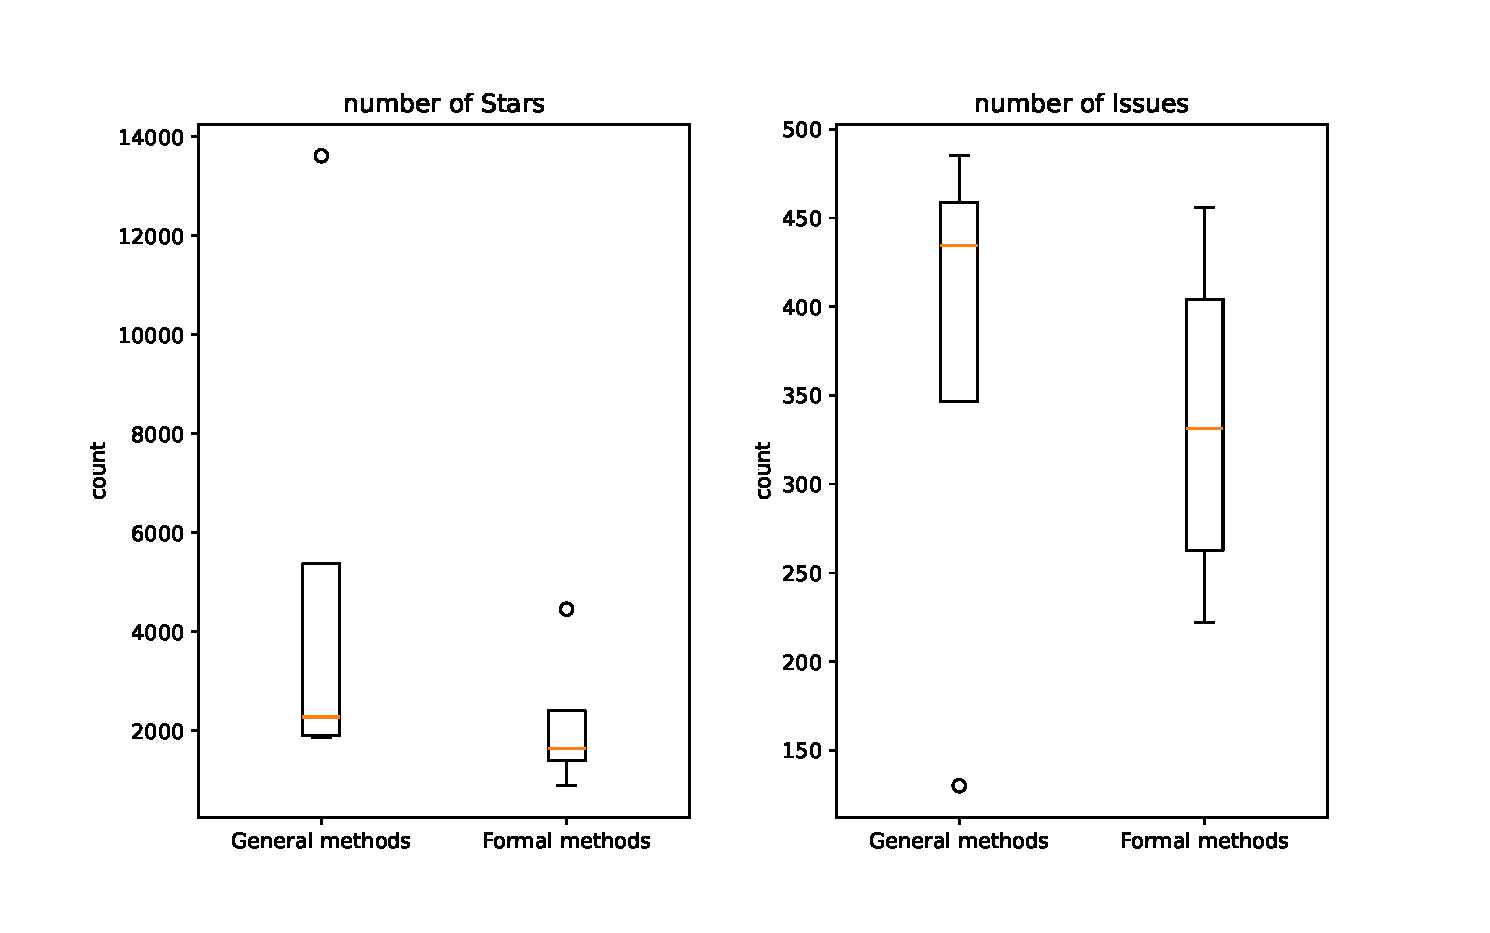
\includegraphics[width=\hsize]{figures/boxplot.eps}
	\caption{形式手法を適用して開発されたリポジトリのデータセットとそうでないリポジトリのデータセットとのIssue数およびStar数の分布}
	\label{fig:boxplot}
\end{figure}

\end{document}
